\section{List of model features/parameters and their biological foundation}
\section{Visual closeness}
\subsection{Ventral Furrow}
After mitosis stops, the the first visual change on the is the belly, where a distinct cleft begins forming. \\

While all cells expressing \textit{twist} \& \textit{snail} lower their apical surface area, they do not constrict indiscriminately, instead starting with the \textit{inner} 8x60 cells.[citation needed] As the furrow closes off, creating closed-off tube with a recognizable light bulb-shape in the cross section, the invaginated tissue "disconnects". This was not part of our simulation.

In figure \ref{fig:VFComparison}, a comparison between

\begin{figure}[H]
    \centering
    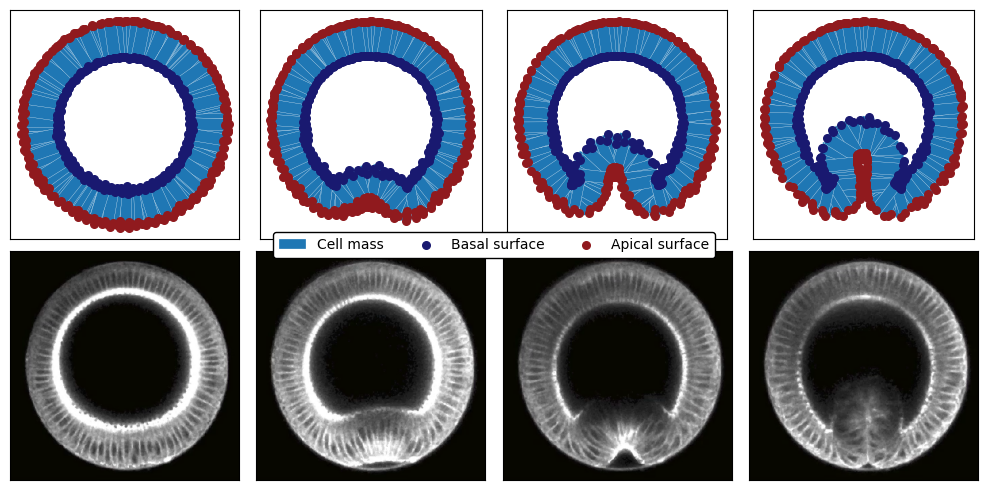
\includegraphics[width=1\linewidth]{chapters/Results/figures/VF_comparison.png}
    \caption{A comparison of simulation and frames from live development. \textbf{Upper row}: Simulation. \textbf{Lower row}: Multi-photon microscopy. \\Each frame is taken at equally spaced time intervals. Cross section video borrowed from \cite{conte2012biomechanical}}
    \label{fig:VFComparison}
\end{figure}


Maybe quantify here?
I am guessing we can do a cell-center fit?
Out of scope? Yes. Would be cool? Also yes.
\subsection{Germ band}
The Germ Band is defined as.

Seeing hwo 

\begin{figure}[H]
    \centering
    \begin{subfigure}[b]{0.25\textwidth}
        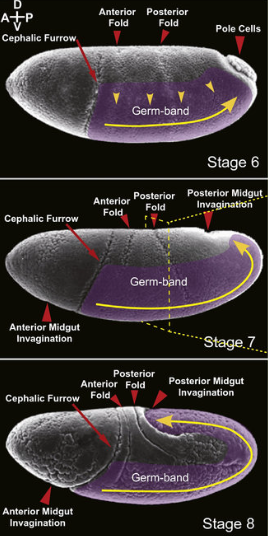
\includegraphics[width=\textwidth]{chapters/Results/figures/compareGB.png}
    \caption{Figure from\cite{kong2017forces} }
        
    \end{subfigure}
     \hfill
    \begin{subfigure}[b]{0.7\textwidth}
    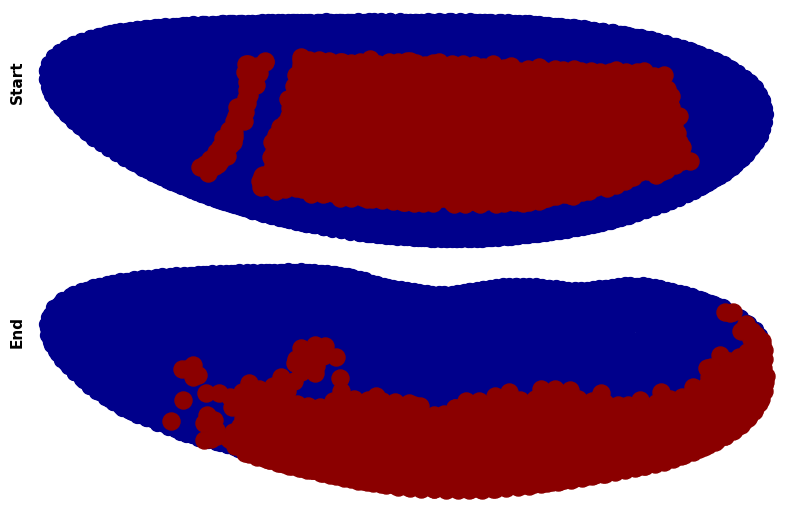
\includegraphics[width=\textwidth]{chapters/Results/figures/gb_firstframe_lastframe.png}
    \caption{Colored in germ band. Elongating posteriorly, moving ventrally.}
    \end{subfigure}
    
\end{figure}


Lorem ipsum dolor 
\\

The individual movements:

\begin{figure}[H]
    \centering
    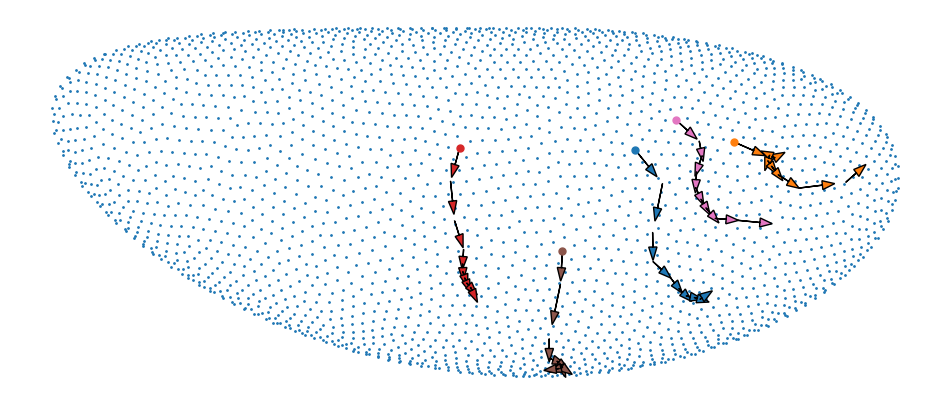
\includegraphics[width=1\linewidth]{chapters/Results/figures/movements.png}
    \caption{NOT TO SELF: Remove some of the cells -- it's cluttered!}
    \label{fig:enter-label}
\end{figure}


\begin{figure}[H]
    \centering
    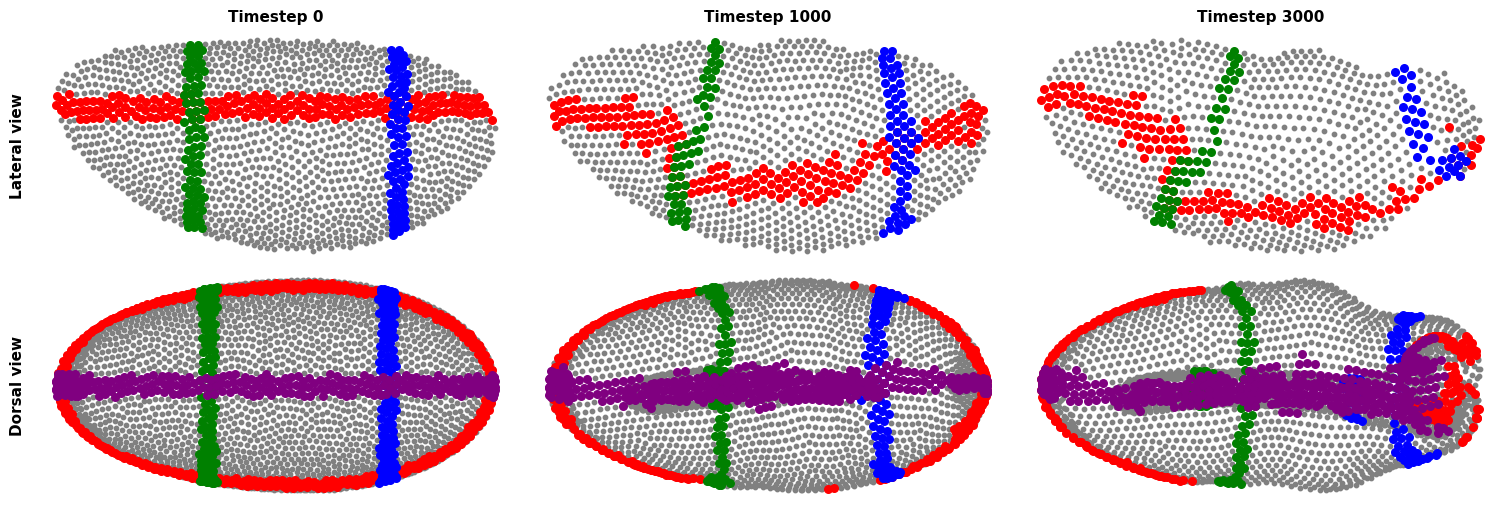
\includegraphics[width=1\linewidth]{chapters/Results/figures/band_movements.png}
    \caption{My simulation. Compare to figure \ref{fig:band-movements-stas}}
    \label{fig:band-movements}
\end{figure}
\begin{figure}[H]
    \centering
    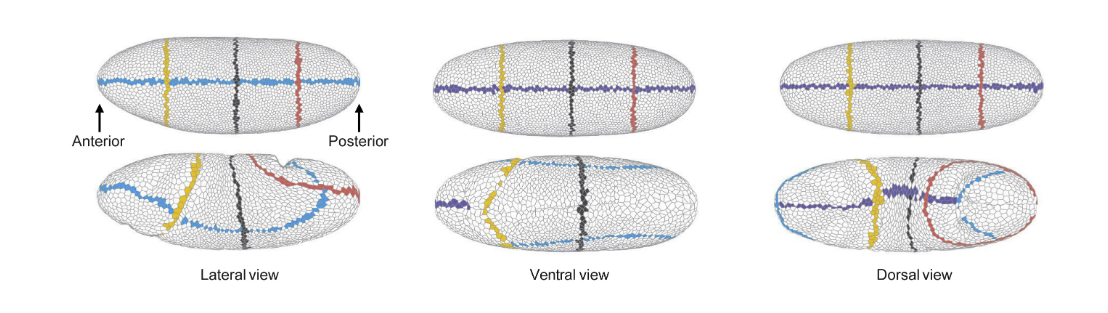
\includegraphics[width=1\linewidth]{chapters/Results/figures/compareStasGBShape.png}
    \caption{Coloured segmented images. Taken from from the brilliant\cite{stern2022deconstructing}. Compare to figure \ref{fig:band-movements}. NOTE TO SELF: Cut only important parts out}
    \label{fig:band-movements-stas}
\end{figure}

% \subsection{Auxiliary furrows}
\subsection{Daniel}
\section{Quantitative closeness}
\subsection{Movements}

\begin{figure}[H]
    \centering
    \makebox[\textwidth][c]{
    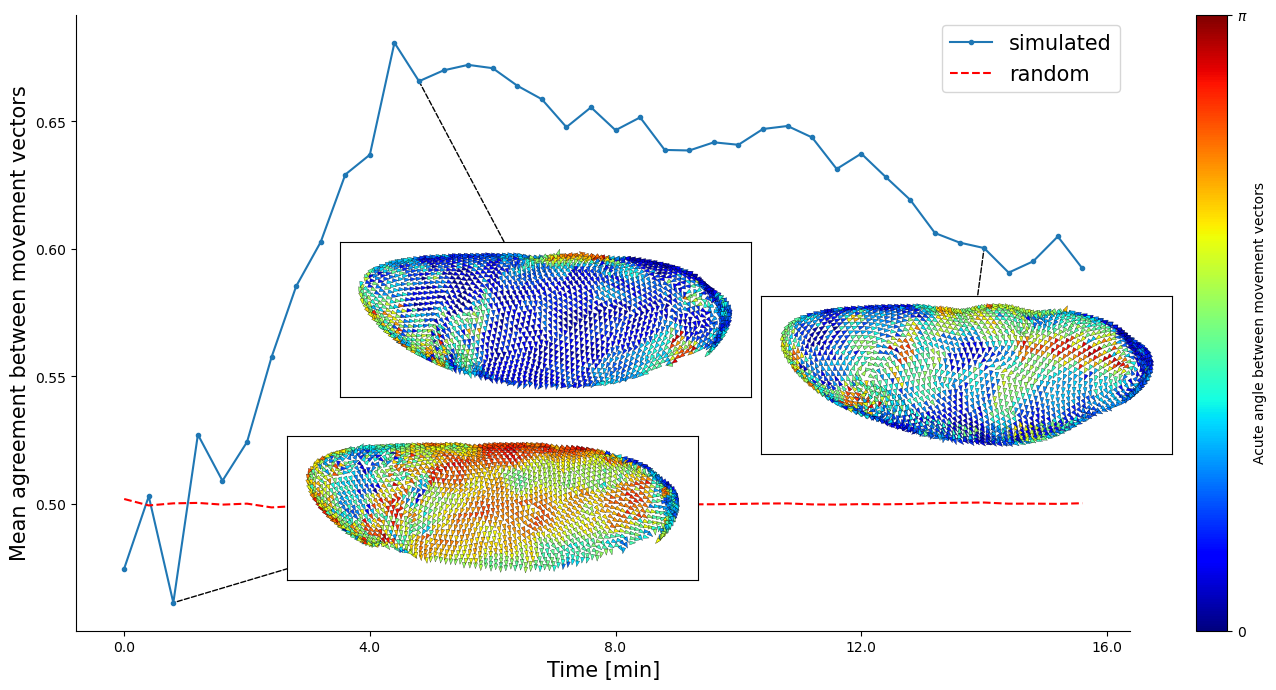
\includegraphics[width=1.3\linewidth]{chapters/Results/figures/movement_vectors_normal.png}
    }
    \caption{Caption}
    \label{fig:enter-label}
\end{figure}

\subsection{Timing}
Even though cells have been shown to have remarkably precise internal clocks\footnote{cool footnote with a remarkable number}\cite{}, there is no evidence for any specific timing in stages 5-7 [citation needed].\textbf{ This is a main result} The fact that we have recapitulated(?) much of the dynamics completely without any explicit time-dependent parameters seems to corroborate our thesis proposed in Section \ref{sec:timedependence}, that Boundary Conditions, Initial Conditions and an inter-atomic rule-set is sufficient for arbitrarily complex morphology/anatomy to arise.\footnote{A sort of Curtis–Hedlund–Lyndon theorem for cells}    

This might be a result of real time 'global' information sharing being limited and not jsut reactions to maternal morphogens.

There is also the "biological clock"\cite{johanolsen2} that proteins themselves have dynamic structure that can change over time.\cite{johanolsen1}
\subsection{Strain}

\subsection{Rosettes}
\begin{figure}[H]
    \centering
    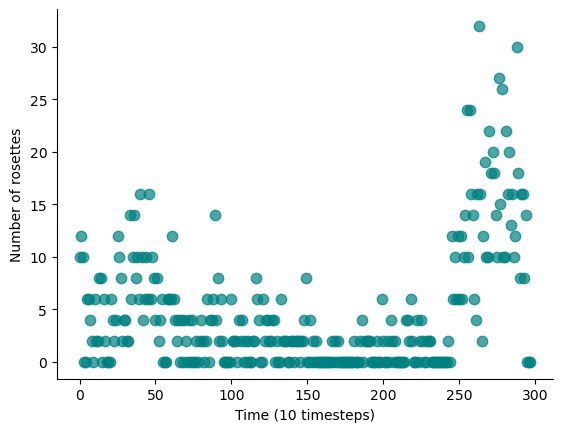
\includegraphics[width=0.5\linewidth]{chapters/Results/figures/rosettes_time.png}
    \caption{Caption}
    \label{fig:enter-label}
\end{figure}

\subsection{Daniel-data?}
\newpage
\section{In Silico Mutant "predictions" - compared to phenotypes and reference model}
\subsection{No PMG}

Knocking out \dots

\begin{figure}[H]
    \centering
    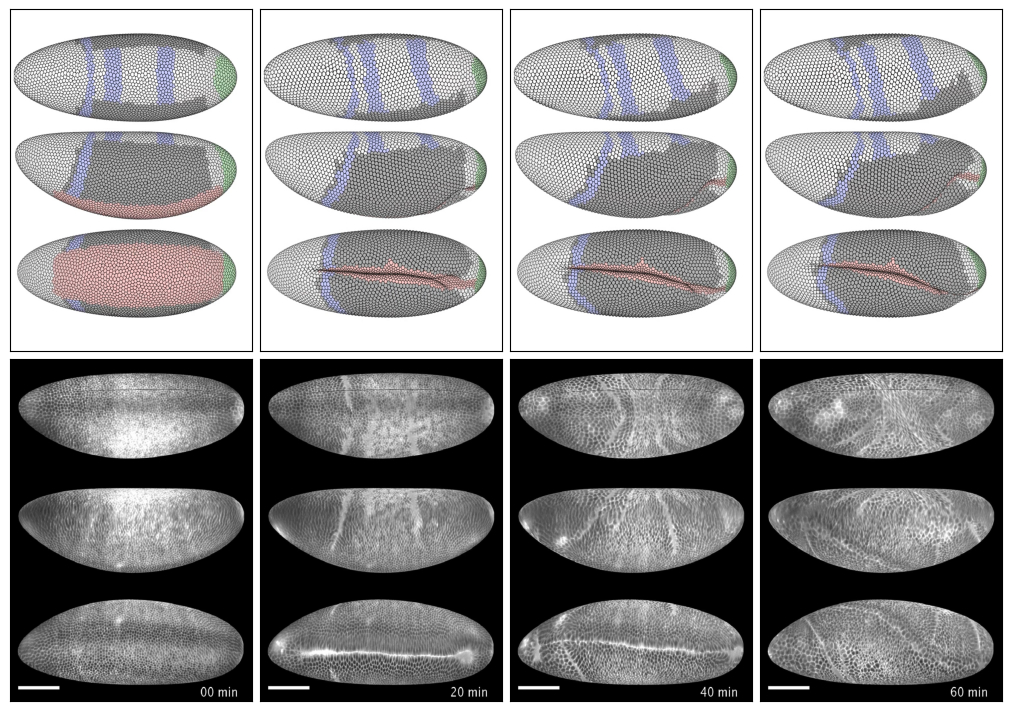
\includegraphics[width=1\linewidth]{chapters/Results/figures/corkscrew_comparison.png}
    \caption{Comparing the \textit{Corkscrew} phenotype with my simulation. Video taken from \cite{smits2023maintaining}}
    \label{fig:corkscrew-comparison}
\end{figure}
% Twist and shout
\subsection{No Ventral Furrow}
% \url{https://genesdev.cshlp.org/content/5/9/1568.full.pdf}
% We are seeing the right thing
\subsection{No Cephalic Furrow?}
% maybe not important
\subsection{No active intercolation / Germ band}
% \url{https://softmath.seas.harvard.edu/wp-content/uploads/2019/10/2009-07.pdf}
% clear that model is missing cell shape change!
\section{Additive/subtractive working together matrix}
% \subsubsection{}